\documentclass[11pt]{article}
\usepackage{upquote}
\usepackage{minted}
\fvset{frame=single}

\usepackage[colorlinks=true]{hyperref}
\usepackage[margin=1in]{geometry}
\usepackage{ifthen}
\usepackage{fancyvrb}

\usepackage{listings}
\usepackage{color}

\definecolor{dkgreen}{rgb}{0,0.6,0}
\definecolor{gray}{rgb}{0.5,0.5,0.5}
\definecolor{mauve}{rgb}{0.58,0,0.82}

\lstset{frame=tb,
  language=Java,
  aboveskip=3mm,
  belowskip=3mm,
  showstringspaces=false,
  columns=flexible,
  basicstyle={\small\ttfamily},
  numbers=none,
  numberstyle=\tiny\color{gray},
  keywordstyle=\color{blue},
  commentstyle=\color{dkgreen},
  stringstyle=\color{mauve},
  breaklines=true,
  breakatwhitespace=true,
  tabsize=3
}

\usepackage{graphicx}
\usepackage{float}

\usepackage{amsmath}
\usepackage{amsfonts}
\usepackage{mathtools}

\usepackage{multirow}
\usepackage{enumitem}

\usepackage{comment}
\usepackage[usenames,dvipsnames,svgnames,table,hyperref]{xcolor}

\newcommand{\vect}[1]{\boldsymbol{#1}}
\newcommand{\matr}[1]{\boldsymbol{#1}}
\DeclareMathOperator*{\argmin}{arg\,min}
\DeclareMathOperator*{\argmax}{arg\,max}
\newcommand{\sol}[1]{{\bf{\color{magenta}{{Solution:}}}}}

\parfillskip=3em plus1fil

\title{CM146, Winter 2023 \\ Problem Set 2: Perceptron and Regression}
\begin{document}

\author{}
\date{}
\vspace{0in}
\maketitle
\vspace{-0.75in}

\section{Perceptron}
\subsection{(a) OR}
\sol x Using T = 1 and F = $-1$, we create the following truth table for $Y = OR(X_1, X_2)$:

\begin{center}
\begin{tabular}{ |c|c|c| }
\hline
X_1 & X_2 & Y \\
\hline
$-1$ & $-1$ & $-1$ \\
$-1$ & $1$ & $1$ \\
$1$ & $-1$ & $1$ \\
$1$ & $1$ & $1$ \\
\hline
\end{tabular}
\end{center}

Plotting this as a graph with $X_1$ as the horizontal axis and $X_2$ as the vertical axis returns points with value $1$ in the first, second, and fourth quadrants, while the point in the third quadrant has value $-1$. We can draw a line that separates the $-1$ data point from the $+1$ data point. Thus, it is linearly separable. If we let $\theta = [w_0, w_1, w_2]^T$, then examples values that work are $\theta = [0.75, 1, 1]^T$ and $\theta = [0.5, 1, 1]^T$.

\subsection{(b) XOR}
\sol x We create the following truth table for $Y = XOR(X_1, X_2)$:

\begin{center}
\begin{tabular}{ |c|c|c| }
\hline
X_1 & X_2 & Y \\
\hline
$-1$ & $-1$ & $-1$ \\
$-1$ & $1$ & $1$ \\
$1$ & $-1$ & $1$ \\
$1$ & $1$ & $-1$ \\
\hline
\end{tabular}
\end{center}

If we plot this as we did with 1.1(a), we see that there is no way to draw a line that separates the +1 and $-1$ data points, so thus, no perceptron exists. We get the following equations:

$$\theta_0 - \theta_1 - \theta_2 < 0$$
$$\theta_0 - \theta_1 + \theta_2 > 0$$
$$\theta_0 + \theta_1 - \theta_2 > 0$$
$$\theta_0 + \theta_1 + \theta_2 < 0$$

\\

Combining the first and fourth equations gives $2\theta_0 < 0$, while combining the second and third equations gives $2\theta_0 > 0$, so the system of equations has no solution.

\section{Logistic Regression}

\subsection{(a) Partial Derivatives}
\sol x Given $J(\boldsymbol{\theta})=-\sum_{n=1}^{N}\left[y_{n} \log h_{\theta}\left(\mathbf{x}_{n}\right)+\left(1-y_{n}\right) \log \left(1-h_{\theta}\left(\mathbf{x}_{n}\right)\right)\right]$, where $h_{\theta}(\mathbf{x})=\sigma(a(\mathbf{x}))$ and $a(\mathbf{x})=\boldsymbol{\theta}^{T} \mathbf{x}+b$. \\

First, get the derivative of $a(\mathbf{x})$ with respect to $\theta_{j}$ :

$$
\frac{d a}{d \theta_{j}}=\frac{d}{d \theta_{j}}\left(\boldsymbol{\theta}^{T} \mathbf{x}+b\right)=x_{j}
$$

Then, find the derivative of $\sigma(a)$ (leaving out the $a$' term that arises from the chain rule):

$$
\frac{d \sigma}{d a}=\frac{d}{d a}\left(\frac{1}{1+e^{-a}}\right)=\frac{0-(1)\left(0+e^{-a}\right)(-1)}{\left(1+e^{-a}\right)^{2}}=\frac{e^{-a}}{\left(1+e^{-a}\right)^{2}}=(\sigma(a))(1-\sigma(a))
$$

Now use these two above results to find the desired answer:
$$
\begin{gathered}
\frac{\partial J}{\partial \theta_{j}}=\frac{\partial}{\partial \theta_{j}}\left(-\sum_{n=1}^{N}\left[y_{n} \log h_{\theta}\left(\mathbf{x}_{n}\right)+\left(1-y_{n}\right) \log \left(1-h_{\theta}\left(\mathbf{x}_{n}\right)\right)\right]\right) \\
=-\sum_{n=1}^{N}\left[y_{n} \frac{\partial}{\partial \theta_{j}}\left(\log h_{\theta}\left(\mathbf{x}_{n}\right)\right)+\left(1-y_{n}\right) \frac{\partial}{\partial \theta_{j}}\left(\log \left(1-h_{\theta}\left(\mathbf{x}_{n}\right)\right)\right)\right] \\
=-\sum_{n=1}^{N}\left[y_{n} \frac{1}{\sigma(a)} \frac{\partial}{\partial \theta_{j}}(\sigma(a))+\left(1-y_{n}\right) \frac{1}{1-\sigma(a)} \frac{\partial}{\partial \theta_{j}}(1-\sigma(a))\right] \\
=-\sum_{n=1}^{N}\left[y_{n} \frac{1}{\sigma(a)} \sigma(a)(1-\sigma(a)) \frac{\partial}{\partial \theta_{j}}\left(a\left(\mathbf{x}_{n}\right)\right)+\left(1-y_{n}\right) \frac{1}{1-\sigma(a)}(-1) \sigma(a)(1-\sigma(a)) \frac{\partial}{\partial \theta_{j}}\left(a\left(\mathbf{x}_{n}\right)\right)\right] \\
=-\sum_{n=1}^{N}\left[y_{n}(1-\sigma(a)) x_{n, j}-\left(1-y_{n}\right) \sigma(a) x_{n, j}\right] \\
=-\sum_{n=1}^{N}\left(y_{n}-\sigma(a)\right) x_{n, j} \\
=\sum_{n=1}^{N}\left(h_{\theta}\left(\mathbf{x}_{n}\right)-y_{n}\right) x_{n, j}
\end{gathered}

\subsection{(b) Hessian}
\sol x To get second partial derivatives, take partial derivative of the obtained equation in 2(a) with respect to $\theta_{k}$ :

$$
\begin{gathered}
\frac{\partial^{2} J}{\partial \theta_{k} \partial \theta_{j}}=\frac{\partial}{\partial \theta_{k}}\left(\sum_{n=1}^{N}\left(h_{\theta}\left(\mathbf{x}_{n}\right)-y_{n}\right) x_{n, j}\right)=\sum_{n=1}^{N} \frac{\partial}{\partial \theta_{k}}\left(h_{\theta}\left(\mathbf{x}_{n}\right)-y_{n}\right) x_{n, j} \\
=\sum_{n=1}^{N} h_{\theta}\left(\mathbf{x}_{n}\right)\left(1-h_{\theta}\left(\mathbf{x}_{n}\right)\right) x_{n, j} x_{n, k}
\end{gathered}
$$

Extending this to all $j, k$ gives us all the entries in the Hessian matrix and the desired result, which can thus be written as:

$$
\mathbf{H}=\sum_{n=1}^{N} h_{\theta}\left(\mathbf{x}_{n}\right)\left(1-h_{\theta}\left(\mathbf{x}_{n}\right)\right) \mathbf{x}_{n} \mathbf{x}_{n}^{T}
$$

\subsection{(c) Convex Function}
\sol x A Hessian is positive semi-definite (PSD) if $\mathbf{z}^{T} \mathbf{H z} \geq 0$ for all real vectors $\mathbf{z}$. Writing it in summation form gives the following:

$$
\mathbf{z}^{T} \mathbf{H z}=\sum_{n=1}^{N} h_{\boldsymbol{\theta}}\left(\mathbf{x}_{n}\right)\left(1-h_{\boldsymbol{\theta}}\left(\mathbf{x}_{n}\right)\right) \mathbf{z}^{T} \mathbf{x}_{n} \mathbf{x}_{n}^{T} \mathbf{z}
$$

Now note that $\mathbf{x}_{n}^{T} \mathbf{z}=\left(\mathbf{z}^{T} \mathbf{x}_{n}\right)^{T}$ and that the expression $\mathbf{x}_{n}^{T} \mathbf{z}$ evaluates to a scalar. If we let this scalar be $p$, we have $\underline{p}^{T}=p$, so thus, $\mathbf{z}_{n}^{T} \mathbf{x}_{n} \mathbf{x}_{n}^{T} \mathbf{z}_{n}=p^{2} \geq 0$. Then, $h_{\boldsymbol{\theta}}\left(\mathbf{x}_{n}\right)$ is restricted to the range $[0,1]$ due to the property of the sigmoid function, and thus so is $\left(1-h_{\theta}\left(\mathbf{x}_{n}\right)\right)$. Thus, the product of all the terms in the summation will be positive, meaning that $\mathbf{z}^{T} \mathbf{H z} \geq 0$ and that the Hessian has been shown to be PSD, which means that $J$ is a convex function, as desired. 

\section{Maximum Likelihood Estimation}

\subsection{(a) Likelihood Function}
\sol x For a Bernoulli distribution, assuming independent and identically distributed (IID),

$$
L(\theta)=P\left(x_{1} ; \theta\right) P\left(x_{2} ; \theta\right) \ldots=\prod_{i=1}^{n} P\left(x_{i} ; \theta\right)=\prod_{i=1}^{n} P\left(\theta^{x_{i}}(1-\theta)^{1-x_{i}}\right)
$$

Because the variables are IID, the likelihood function does not depend on the order in that the random variables are observed.

\subsection{(b) MLE}
\sol x Taking the log of both sides to get the log likelihood:

$$
\begin{gathered}
l(\theta)=\log \left(\prod_{i=1}^{n} P\left(x_{i} ; \theta\right)\right)=\sum_{i=1}^{N} \log P\left(x_{i} ; \theta\right)=\sum_{i=1}^{N} \log P\left(\theta^{x_{i}}(1-\theta)^{1-x_{i}}\right) \\
=\sum_{i=1}^{N}\left[x_{i} \log \theta+\left(1-x_{i}\right) \log (1-\theta)\right]
\end{gathered}
$$

First and second derivatives:

$$
\begin{gathered}
\frac{d l}{d \theta}=\frac{d}{d \theta} \sum_{i=1}^{N}\left[x_{i} \log \theta+\left(1-x_{i}\right) \log (1-\theta)\right] \\
\frac{d l}{d \theta}=\sum_{i=1}^{N}\left[\frac{x_{i}}{\theta}-\frac{1-x_{i}}{1-\theta}\right] \\
\frac{d^{2} l}{d \theta^{2}}=\frac{d}{d \theta} \sum_{i=1}^{N}\left[\frac{x_{i}}{\theta}-\frac{\left(1-x_{i}\right)}{(1-\theta)}\right]=\sum_{i=1}^{N}\left[-\frac{x_{i}}{\theta^{2}}-\frac{(-1)\left(1-x_{i}\right)(-1)}{(1-\theta)^{2}}\right] \\
\frac{d^{2} l}{d \theta^{2}}=\sum_{i=1}^{N}\left[-\frac{x_{i}}{\theta^{2}}-\frac{1-x_{i}}{(1-\theta)^{2}}\right]
\end{gathered}
$$

Letting the sum of $x_{i}$ over all $i$ equal $x_{\text {total, }}$ setting the first derivative equal to 0 and solving for $\theta$:

$$
\begin{aligned}
& \sum_{i=1}^{N}\left[\frac{x_{i}}{\theta}-\frac{1-x_{i}}{1-\theta}\right]=0 \\
& \sum_{i=1}^{N} \frac{x_{i}}{\theta}=\sum_{i=1}^{N} \frac{1-x_{i}}{1-\theta} \\
& \frac{x_{\mathrm{total}}}{\theta}=\frac{N-x_{\mathrm{total}}}{1-\theta} \\
& x_{\mathrm{total}}=N \theta \\
& \theta=\bar{x}
\end{aligned}
$$

\subsection{(c) Likelihood plot $\theta$}
\sol x \begin{center}
    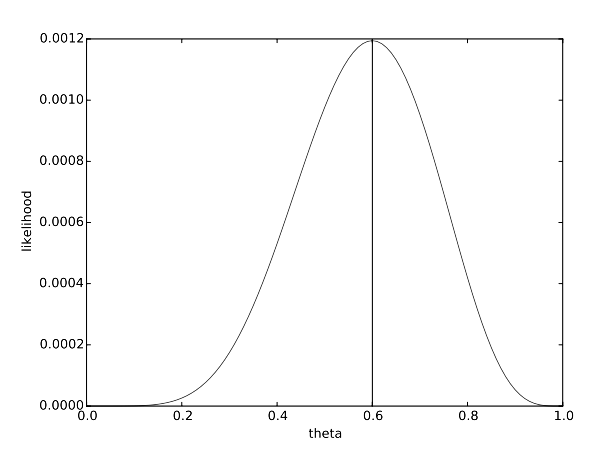
\includegraphics[scale=0.4]{3c.png} \\
\end{center}

The value of $\theta$ that seems to maximize the likelihood is $0.6$, which agrees with what I obtained using the result of 3(b).

\subsection{(d) Likelihood plot Data}
\sol x For $n=5$, with three 1s and two 0s:

\begin{center}
    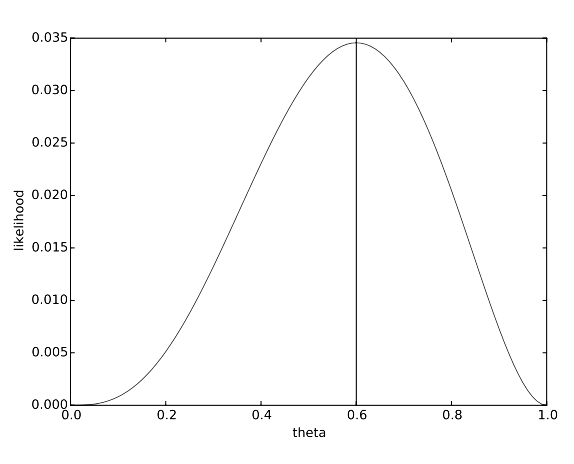
\includegraphics[scale=0.4]{3d-1.png} \\
\end{center}

The graph is centered at $\theta=0.6$, which is the same as the graph in 3(c), and it has the same bell curve shape. However, due to $n$ being smaller (5 versus 10 for 3(c)), the standard deviation (spread) of the results is higher. Graphically, the bell curve is wider. Also, compared to $n=10$, the maximum likelihood value is higher (about $0.035$ versus about $0.0012$ from 3(c)). \\

For $n=100$, with sixty 1s and forty 0s:

\begin{center}
    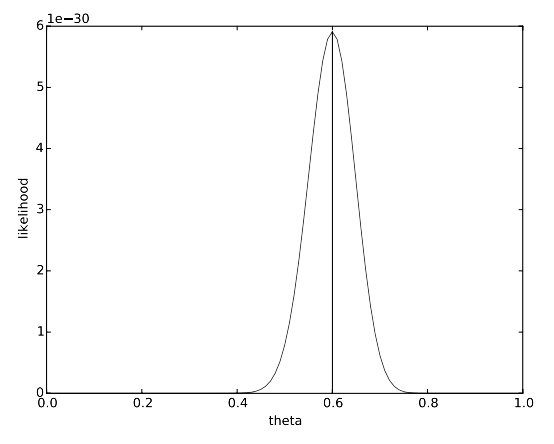
\includegraphics[scale=0.4]{3d-2.png} \\
\end{center}

This graph is centered at $\theta=0.6$, which is the same as the two previous graphs, and it still has the bell curve shape, but due to $n$ increasing to 100, the width of the bell curve is much less (meaning $L(\theta)$ has a lower standard deviation). Also, the maximum likelihood value is much lower this time, on the order of $10^{-30}$, compared to $0.035$ for $n=5$ and $0.0012$ for $n=10$. \\

For $n=10$, with five 1s and five 0s:

\begin{center}
    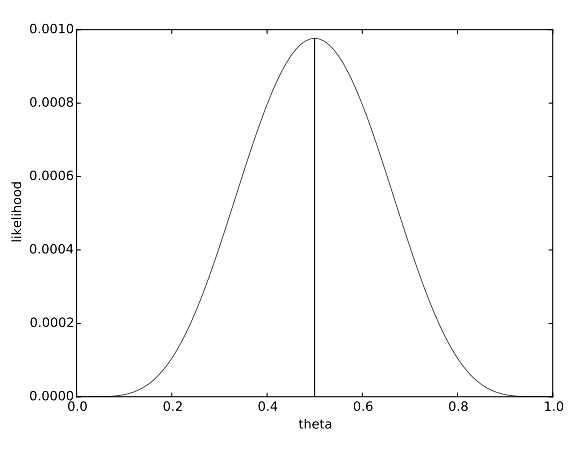
\includegraphics[scale=0.4]{3d-3.png} \\
\end{center}

This time, unlike the other 3 preceding graphs, this one is centered at $\theta=0.5$, but it still has the same bell curve shape as all the other graphs. The spread seems to be roughly the same as the graph in 3(c). The maximum likelihood value is roughly the same in the graph for 3(c): this one is roughly $0.0010$, while for $3(\mathrm{c})$ it is $0.0012$. \\

Concluding remarks: It looks like $n$ affects standard deviation: as $n$ increases, standard deviation decreases. The graph is centered about the proportion of ones in the data set. The tendency of the curve to look like the normal curve as $n$ increases is due to the central limit theorem. Essentially, as the number of samples n increases, the likelihood function gets more peaked at its maximum value, and the values it takes on decrease.

\section{Linear and Polynomial Regression}

\subsection{(a) Visualization}
\sol x The training data is slightly noisy and shows a weak negative correlation between X and y. On the other hand, the test data is extremely noisy, showing that polynomial regression might fit the test data better than linear regression. In order, the following graphics depict the training data and test data.

\begin{center}
    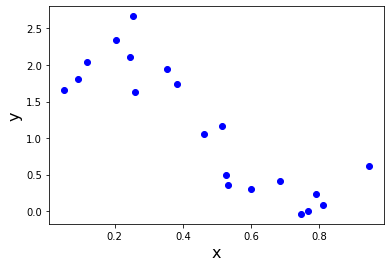
\includegraphics[scale=0.5]{4a-1.png}
    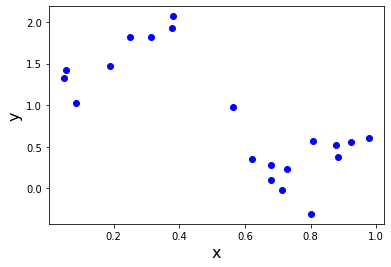
\includegraphics[scale=0.5]{4a-2.png}
\end{center}


\subsection{(b) Constructing X}
\sol x \begin{lstlisting}
### ========== TODO : START ========== ###
# part b: modify to create matrix for simple linear model
    Phi = np.append(np.ones([n, 1]), X, 1)
### ========== TODO : END ========== ###
\end{lstlisting}

\subsection{(c) Prediction}
\sol x 
\begin{lstlisting}
### ========== TODO : START ========== ###
# part c: predict y
    y = np.dot(X, np.transpose(self.coef_))
### ========== TODO : END ========== ###
\end{lstlisting}

\subsection{(d) Gradient Descent}
\sol x 
\begin{lstlisting}
### ========== TODO : START ========== ###
# part d: compute J(theta)
    y_predicted = self.predict(X)
    n,d = X.shape
    cost = 0
    for i in range(len(X)):
    cost += (y_predicted.flat[i] - y[i]) ** 2
### ========== TODO : END ========== ###
\end{lstlisting}

\begin{lstlisting}
### ========== TODO : START ========== ###
# part d: update theta (self.coef_) using one step of GD
# hint: you can write simultaneously update all theta using vector math
                
# track error
# hint: you cannot use self.predict(...) to make the predictions
    y_pred = np.dot(X, self.coef_) # change this line
# cannot use self.predict() because that refits the data
# print str(X)
    grad_res = np.dot(y_pred-y, X) #y-hat minus y, multiplied by xj
    self.coef_ = self.coef_ - 2 * eta * grad_res # update J(theta)
    err_list[t] = np.sum(np.power(y - y_pred, 2)) / float(n)                 
### ========== TODO : END ========== ###
\end{lstlisting}

\begin{center}
\begin{tabular}{|l|l|l|l|l|}
\hline${\text { Step Size, } \eta}$ & \multicolumn{1}{|c|}{${\theta_{0}}$} & \multicolumn{1}{c|}{${\theta}_{1}$} & ${\text { Iterations }}$ & ${\text { Cost }}$ \\
\hline $10^{-4}$ & $2.27045$ & $-2.46068$ & 10000 & 4.0864 \\
\hline $10^{-3}$ & $2.44641$ & $-2.81635$ & 7020 & 3.91258 \\
\hline $10^{-2}$ & $2.44641$ & $-2.81635$ & 764 & 3.91258 \\
\hline $10^{-1}$ & NaN & NaN & 10000 & NaN \\
\hline
\end{tabular}
\end{center}

The results show that for a step size of around $10^{-2}$ does the best, and that $10^{-3}$ is a bit small but still large enough to converge within 10,000 iterations. However, when the step size is $10^{-4}$, it is too small and takes too long to converge, as it reaches the 10,000 iterations limit. On the other hand, $0.1$ is too large of a step size, as it also reaches the 10,000 iterations limit but the coefficients are very different from the other step sizes (numerically instable), indicating that the line is very likely to be incorrect. The step size is too large for the algorithm to converge. For the coefficients, it seems that the algorithm causes the coefficients to converge to roughly $\theta_{0}=2.44641$ and $\theta_{1}=-2.81635$, with the results for $\eta=10^{-3}$ being very close to the results for $\eta=10^{-2}$. For $\eta=10^{-4}$, it started making progress towards the values reported for $\eta=10^{-2}$, but the step size was too small for a limit of 10,000 iterations, and so it wasn't able to reach the final values. And as previously stated, for $\eta=0.1$, the step size was too big, and so it never converged and thus reported numerical instability.

\subsection{(e) Closed form}
\sol x
\begin{lstlisting}
### ========== TODO : START ========== ###
# part e: implement closed-form solution
    xt_x = np.dot(np.transpose(X),X)
    self.coef_ = np.dot(np.dot(np.linalg.pinv(xt_x),np.transpose(X)),y)
    return self
### ========== TODO : END ========== ###
\end{lstlisting}

The closed form solution is $\theta_{0}=2.446407$ and $\theta_{1}=-2.816353$, and the cost is 3.912576. For gradient descent with smaller step sizes, the coefficients are closer to the closed-form solution. In this case, the closed-form solution is faster than gradient descent, since it takes 0.00117 seconds to run, versus GD's 0.12098 seconds.

\subsection{(f) Auto Learning Rate}
\sol x 
\begin{lstlisting}
### ========== TODO : START ========== ###
# part f: update step size
# change the default eta in the function signature to 'eta=None'
# and update the line below to your learning rate function
    if eta_input is None :
        eta = float(1)/(1+t) # change this line
    else :
        eta = eta_input
### ========== TODO : END ========== ###
\end{lstlisting}

Using an iterative step size, the runtime decreases to $0.068$s, with the algorithm converging in 1511 iterations to values of $\theta_{0}=2.44641$ and $\theta_{1}=-2.81635$, essentially the same as the results in part (d) (note: rounded to 5 decimal places). The cost remains the same too. As the iteration number increases, the step size decreases, so thus, at the start, the algorithm quickly moves towards the minimum, and as it gets closer, it decreases its step size.

\subsection{(g) Constructing polynomial X}
\sol x
\begin{lstlisting}
### ========== TODO : START ========== ###
# part g: modify to create matrix for polynomial model
    Phi = []
    m = self.m_
    for i in range(m + 1):
        Phi.append(X.reshape((-1,)) ** i)
    Phi = np.array(Phi)
    Phi = np.transpose(Phi)
### ========== TODO : END ========== ###
\end{lstlisting}

\subsection{(h) RMSE}
\sol x
\begin{lstlisting}
### ========== TODO : START ========== ###
# part h: compute RMSE
    error = 0
    error = np.sqrt(self.cost(X, y)/X.shape[0])
### ========== TODO : END ========== ###
\end{lstlisting}

Because RMSE involves division by the number of data points, it eliminates the size of a data set as a factor affecting the magnitude of error. It also represents the sample standard deviation of the residuals and is therefore on the same scale as the predictions (opposed to sample variance). 

\subsection{(i) Model Complexity}
\sol x

For $m < 3$, there is evidence of underfitting, since the training error is very high in comparison to test error. The minimum test error occurs with a polynomial of degree 5. Underfitting can be seen on the left, where both the test and training errors are similarly high (in the neighborhood of $0.75$ to 1). Then, as the degree of the polynomial increases (the model's complexity), the training error monotonically decreases, while the test error first decreases, and then suddenly increases at the end. The test error reaches its minimum at degree 5, as mentioned above, and the sudden increase in error as the degree becomes high while training error is low is a sign of overfitting. We can derive that 4-6th degree polynomials fit the data best. For $m > 8$, there is evidence of overfitting, essentially, the test error increases greatly but training error decreases.

\begin{center}
    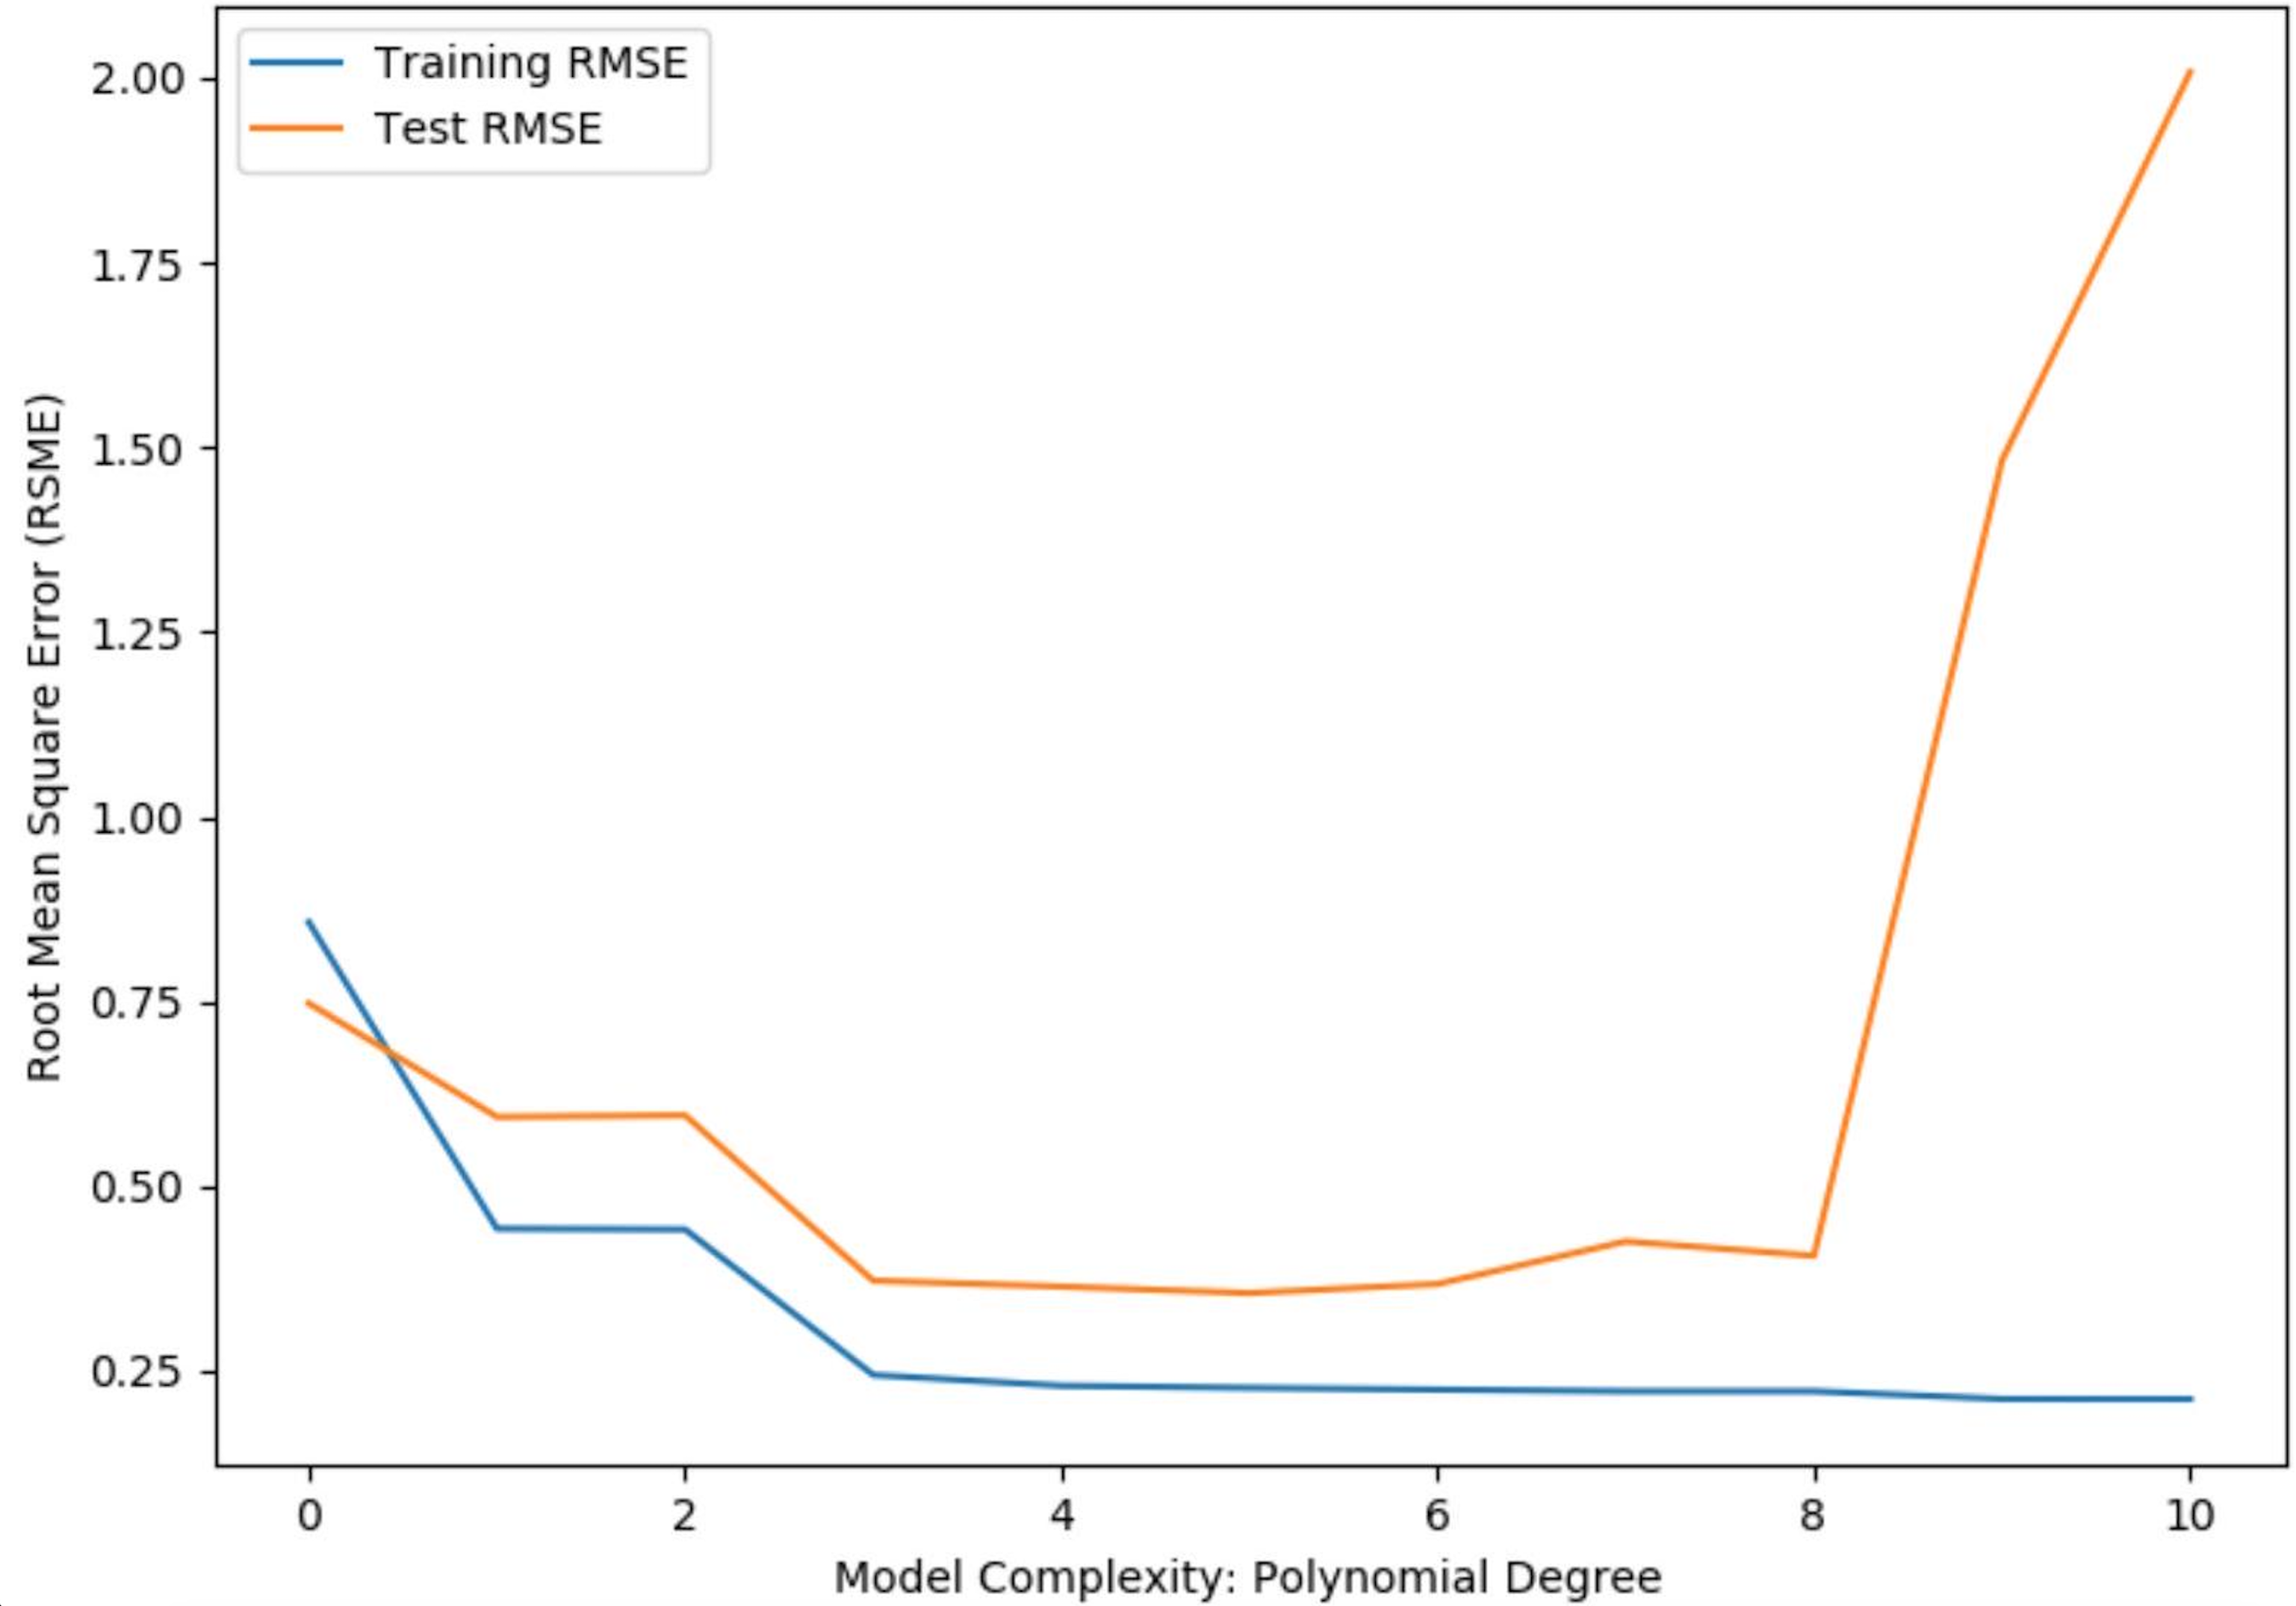
\includegraphics[scale=0.16]{4i.png}
\end{center}

\end{document}